\documentclass[11.5pt]{sig-alternate} % sets document style to sig-alternate
% packages
% typesetting
%\usepackage{dirtytalk} % typset quotations easier (\say{stuff})
\usepackage{hanging} % hanging paragraphs
\usepackage[defaultlines=3,all]{nowidow} % avoid widows
\usepackage[pdfpagelabels=false]{hyperref} % produce hypertext links, includes backref and nameref
\usepackage{xurl} % defines url linebreaks, loads url package
\usepackage{microtype}
%\usepackage[super]{nth} % easily create superscript ordinal numbers with \nth{x}
\usepackage{textcomp}
\newcommand{\texttildemid}{\raisebox{0.4ex}{\texttildelow}}
% layout
%\usepackage{enumitem} % control layout of itemize, enumerate, description
\usepackage{fancyhdr} % control page headers and footers
\usepackage{float} % improved interface for floating objects
%\usepackage{multicol} % intermix single and multiple column pages
% language
\usepackage[utf8]{inputenc} % accept different input encodings
\usepackage[english]{babel} % multilanguage support
% misc
\usepackage{graphicx} % builds upon graphics package, \includegraphics
%\usepackage{lastpage} % reference number of pages
%\usepackage{comment} % exclude portions of text (?)
\usepackage{xcolor} % color extensions
\usepackage[backend=biber, style=apa]{biblatex} % sophisticated bibliographies % necessary for HTML to display author info and date on abstract page
\usepackage{csquotes} % advanced quotations, makes biblatex happy
\usepackage{authblk} % support for footnote style author/affiliation
% tables and figures
\usepackage{tabularray}
%\usepackage{array} % extend array and tabular environments
\usepackage{caption} % customize captions in figures and tables (rotating captions, sideways captions, etc)
%\usepackage{cuted} % allow mixing of \onecolumn and \twocolumn on same page
\usepackage{multirow} % create tabular cells spanning multiple rows
%\usepackage{subfigure} % deprecated, support for manipulation of small figures
%\usepackage{tabularx} % extension of tabular with column designator "x", creates paragraph-like column whose width automatically expands
%\usepackage{wrapfig} % allows figures or tables to have text wrapped around them
%\usepackage{booktabs} % better rules
% dummy text
%\usepackage{blindtext} % blind text dummy text
%\usepackage{kantlipsum} % Kant style dummy text
\usepackage{lipsum} %lorem ipsum dummy text
% other helpful packages may be booktabs, longtable, longtabu, microtype

\pagestyle{fancy} % sets pagestyle to fancy for fancy headers and footers

% header and footer
% modern way to set header image
\renewcommand{\headrulewidth}{0pt} % defines thickness of line under header
\renewcommand{\footrulewidth}{0pt} % defines thickness of line above header
\setlength\headheight{80.0pt} % sets height between top margin and header image, effectively moves page contents down
\addtolength{\textheight}{-80.0pt} % seems to affect the lower height. maybe only works properly if footer numbers enabled?
\fancyhf{}
\fancyhead[CE, CO]{
\includegraphics[width=\textwidth]{headerImage.png}}
% footer
%\fancyfoot[LE,LO]{Article Title Here \\ DOI: }% left footer article title and doi
%\fancyfoot[CE,CO]{{}} % center footer empty
%\fancyfoot[RE,RO]{\thepage} % right footer page numbers
%\pagenumbering{arabic} % arabic (1, 2, 3) numbering in footer

\hypersetup{colorlinks=true,urlcolor=blue} % sets link color to blue
\urlstyle{same} % sets url typeface to same as rest of text

% set caption and figure to italics, label bold, left align captions, does not transfer to HTML
\captionsetup{labelfont=bf, font={large, it}, justification=raggedright, singlelinecheck=false}
\renewcommand\theContinuedFloat{\alph{ContinuedFloat}}

%this next bit is confusing, but essentially changes the width of the abstract. Seems to have been copied from this https://tex.stackexchange.com/questions/151583/how-to-adjust-the-width-of-abstract
\let\oldabstract\abstract
\let\oldendabstract\endabstract
\makeatletter %changes @ catcode to enable modification (in parsep)
\renewenvironment{abstract} %alters the abstract environment
{\renewenvironment{quotation}%
               {\list{}{\addtolength{\leftmargin}{1em} % change this value to add or remove length to the the default ?
                        \listparindent 1.5em%
                        \itemindent    \listparindent%
                        \rightmargin   \leftmargin%
                        \parsep        \z@ \@plus\p@}%
                \item\relax}%
               {\endlist}%
\oldabstract}
{\oldendabstract}
\makeatother %changes @ catcode to disable modification

% checks
% italics -
% links -
% dashes -
% tildes -
\begin{document}

\title{Teaching Basic Cryptography Concepts Using Braille and Large Print Manipulatives}

\author[1]{\large \color{blue}Jason Martin }

\affil[1]{Alabama Department of Rehabilitation Services}

\toappear{}
%% ABSTRACT
\maketitle
\begin{@twocolumnfalse} 
\begin{abstract}
\item 
\textit {The scope of this article is to describe the creation and implementation of specialized adaptations used in teaching the subject of basic cryptography to students who are visually impaired or blind. Included is an overview of events held for visually impaired and blind transition age youth in Alabama and the methods used to engage this population in the subject of computer science. Teaching strategies utilized for this unique demographic of students are discussed as they relate to the sample  cryptography lessons used during the transition day events. The construction of  three forms of adapted ciphers are described in addition to general information about modifications. Limitations encountered with specific designs, such as braille tracking issues, are also conveyed. The manipulative designs suggested in this article fulfilled a specific need and allowed participants with varying degrees of visual impairments to complete the process of encryption and decryption. Further evidence to suggest proven effectiveness of the manipulatives is needed as the initial designs are intentionally low cost and rudimentary in nature.}
\\ \\
Keywords: Braille, Cryptography, Visual Impairments, Blind, Computer Science 
\end{abstract}
\end{@twocolumnfalse}

%% AUTHOR INFORMATION

\textbf{*Corresponding Author, Jason Martin}\\
\href{mailto: jason.martin@rehab.alabama.gov }{(jason.martin@rehab.alabama.gov)} \\
\textit{Submitted February 11th, 2019 }\\
\textit{Accepted March 28th, 2019} \\
\textit{Published online April 8th, 2019} \\
\textit{DOI:10.14448/jsesd.11.0007} \\
\pagebreak
\clearpage

\begin{large}
\section*{INTRODUCTION}

Segments of the NSA Gencyber program (GenCyber, 2017) served as the basis for the curriculum of a specialized transition program for youth who are visually impaired or blind. Developed by the Alabama Institute for Deaf and Blind in partnership with the Alabama Department of Rehabilitation Services the program, “STEM WARS Vol. 2: Guardians of the Cyber Galaxy,” was held on five separate college campuses across Alabama with an attendance of seventy six student participants overall (Beavers, 2018, June). To encourage student engagement, the program integrated themes from popular comic book films with cybersecurity principles, encouraged engagement from visually impaired mentors, included presentations from academic and experienced  professionals, and incorporated project based learning with friendly competition. The following reflects the methods and adaptations used in developing one of the core instructional  lessons taught during this program.      

\section*{OVERVIEW}

The basis for the lesson “Cryptography Basics,”  was provided by the University of Alabama Huntsville during a previous collaboration with the Alabama Institute for Deaf and Blind, where the Gencyber program was adapted for students who were Deaf or Hard of Hearing (Hairston, 2017, June). This fundamental portion of the lesson provided students with introductory knowledge of cryptography, how cryptography is used by everyone, a brief history of encryption, and various methods of encryption. During the second portion of the lesson, “Groot’s Password Problem,”  students were given individual adapted Caesar ciphers to complete two sample encryption scenarios and were provided problem samples in large print and braille (Martin, 2018, April).. The scenarios were themed with satirical social engineering issues featuring characters from the film “Guardians of the Galaxy,” (Gunn et al, 2014) Students were guided through the first scenario and were timed during the second. Timed scores were used to determine performance for teams during the ending awards portion of the day event.

\section*{METHOD}

While presenting both sections of this lesson, all slides were read aloud and all images were verbally described in detail. Students were allowed to respond after each slide of material was covered, creating a dialogue around each individual point.  Models for historical ciphers referenced were created as lesson manipulatives. The replica of the Scatyle (Hairston, 2017, June) was created by wrapping a long strip, approximately 1x14 in. of paper around a light foam plastic rod, approximately 3 x 12 inches. The unencrypted message was written across the paper horizontally and then unrolled from the rod. The unrolled handwritten ciphertext was then transcribed into a digital template to modify various aspects of the text including font and color density. Each letter of the clearly printed version of the ciphertext was then embossed in braille, using a Perkins Braille Writer, to create a manipulative that worked for both groups of students.

\begin{figure}[!h]
    \centering
    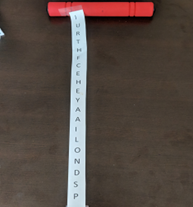
\includegraphics[width=1\linewidth]{images/fig1.png}
    \caption{Image of the Scatlye manipulative with enlarged and modified sample text unfurled.}
\end{figure}
 
\begin{figure}[!h]
    \centering
    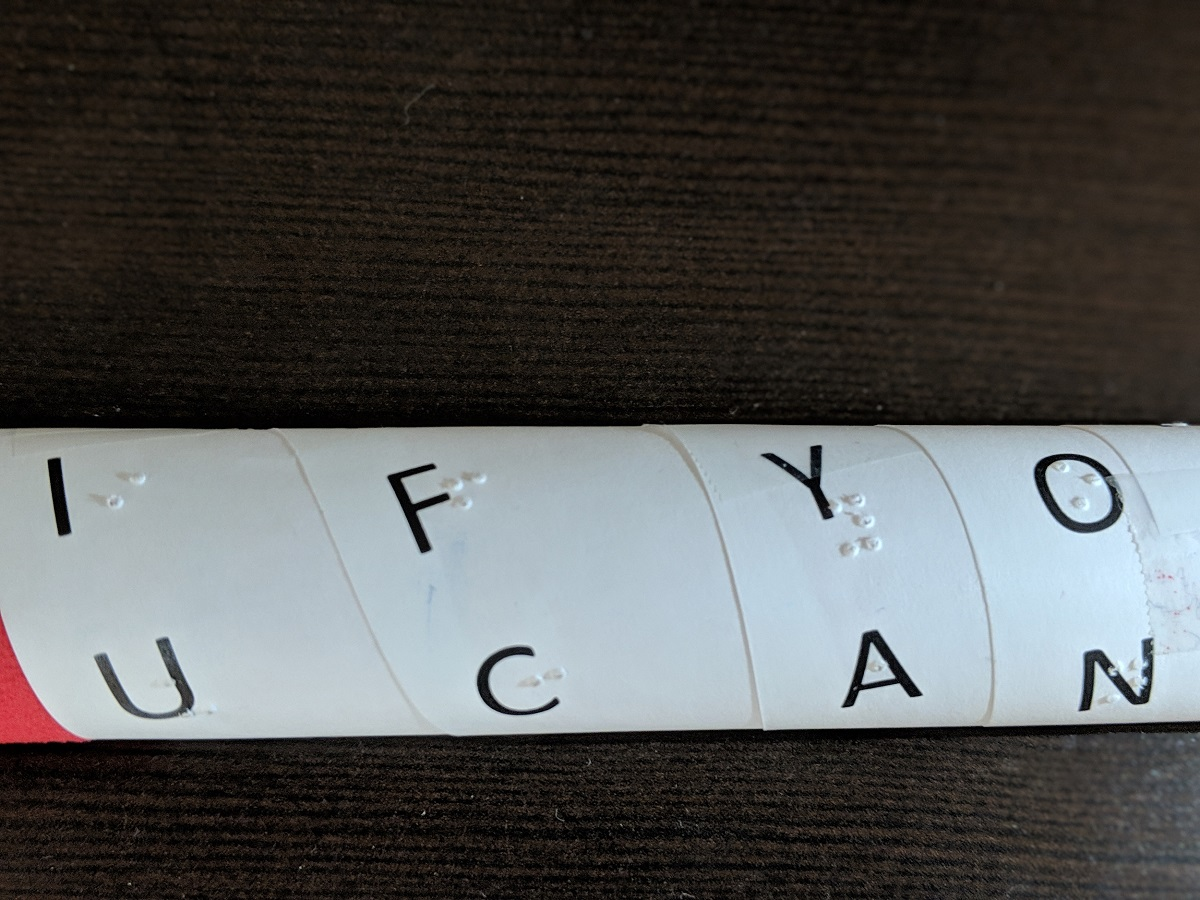
\includegraphics[width=1\linewidth]{images/fig2.jpg}
    \caption{Close up on the Scatyle manipulative. The message is wrapped around the rod and the words “If You Can” can be made out. Spacing is atypical because of the nature of the particular type of cipher. Embossed braille can be read over or near  each letter.}
\end{figure}

The model of the Caesar cipher was created from a template worksheet (Clark, 2013) and was modified into three different versions. The basic model of the Caesar cipher consisted of one small and one large rotating  paper circle printed with the complete alphabet on the outer rim of each.  The center of the circles were connected using a standard office supply binder clip. The high contrast cipher model was developed as an alteration to the original design by replacing the alphabet with bold and large printed font on a white background. The inner ring was also modified by using black font on yellow paper to offer a contrast that allowed students to easily differentiates the inside portion from the outside portion of the ring. 
 
\begin{figure}[!h]
    \centering
    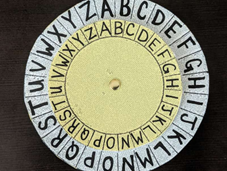
\includegraphics[width=1\linewidth]{images/fig3.png}
    \caption{An image of a high contrast version of the Caesar cipher. The template was printed and glued to two paper plates, one small and one large. Lettering on the outside of each ring of the cipher was darkened and yellow paper was used in the center to provide contrast.}
\end{figure}

A version of the high contrast cipher was also labeled in braille; however, this particular adaptation proved to be problematic for effective tracking and frequently moved while in use. An alternative solution to the Caesar cipher manipulative for braille users was developed to simplify the encryption exercise. “Cipher Sticks,” were the result of printing copies of the braille alphabet on linear strips and affixing that alphabet to a thick cardboard  backing with rubberized non-slip material attached to the back of each stick. 

\begin{figure}[!h]
     \centering
     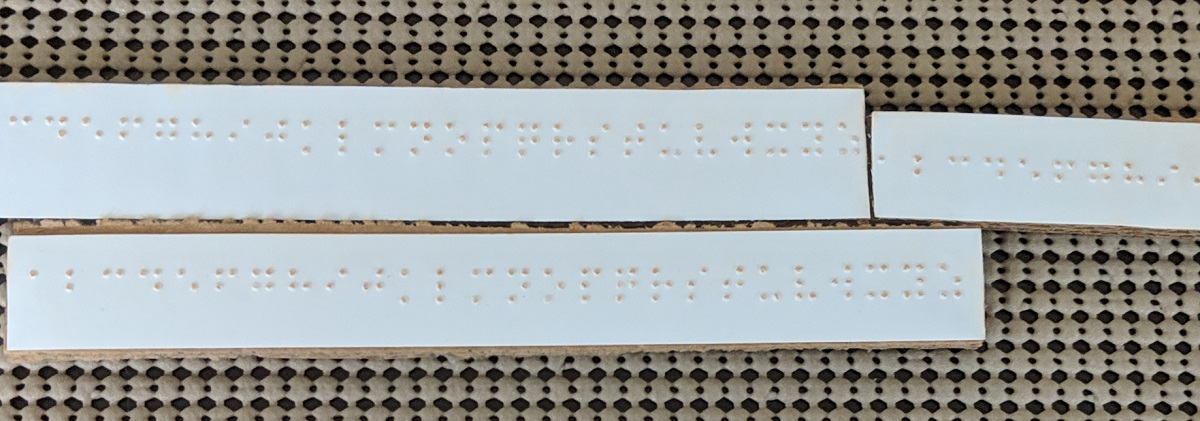
\includegraphics[width=1\linewidth]{images/fig4.jpg}
     \caption{Image of “Cipher Sticks.” The braille in this photo has been shaded for image clarity. In this example the A on the bottom stick corresponds to the C on the top row. Every letter can now be easily read and corresponds with a shift of two.}
 \end{figure} 

These ciphers were expanded designs of the example linear cipher within the sample worksheet template (Clark, D.R., 2013). Each alphabet stick had a thin margin next to the letters A and Z to allow for appropriate tracking when making the connection of a second cipher stick on either end. The student would then place a third cipher stick, underneath the appropriate “key” letter of the first line and would read the corresponding two lines to encrypt or decrypt information. During the program, this method proved to be the most effective means for readers of braille to complete the sample exercises comparable to their peers with visual impairments.

\section*{CONCLUSION}

The adaptations created for use within this specialized program were exploratory in nature and the initial rudimentary designs of the manipulatives have substantial room for improvement. In the absence of a specific existing product, this basic design allowed all students in attendance to actively participate in the lessons designed to teach  cryptography basics. The low cost design of the manipulatives used were intentionally constructed of craft materials to afford students and instructors a low barrier of entry to participate. Students were also allowed to keep the adapted ciphers and were encouraged to continue encryption exercises with peer groups. While the prototype versions of the adapted ciphers were momentarily sufficient, future manipulative designs will require significantly more formal testing and evidence based research to derive a proven and effective method for teaching cryptography.  

\end{large}
\clearpage
\section*{REFERENCES}\par 

\leftskip 0.25in
\parindent -0.25in 
Clark, D. R. (2013). Cryptography Worksheet — The Caesar Shift [PDF]. \url{https://crypto.interactive-maths.com/}.

Beavers, I. (2018, June). [Attendance of College Transition Day Students]. Unpublished raw data.

GenCyber. (2017). Retrieved January 11, 2019, from \url{https://www.gen-cyber.com/}

Gunn, J. (Director), Gunn, J., Perlman, N., Diesel, V., \& Cooper, B. (Writers), \& Feige, K. (Producer). (2014). Guardians of the Galaxy[Video file]. United States: Walt Disney Studios Motion Pictures.

Hairston, J. (2017, June). Cryptography Basics. Lecture presented at Gencyber Camp for Teachers of Deaf and Hard of Hearing Students in University of Alabama Huntsville, Huntsville.

Figure 1,2,3,4. [Personal photographs taken in Montgomery, Alabama]. (2019, February 12).

Martin, J. M. (2018, April). Groot Password Problem. Lecture presented at STEM Wars Vol. 2. in Bishop State, Mobile.

\end{document}